\begin{figure}[t]
  \centering
  \vspace{8pt}
  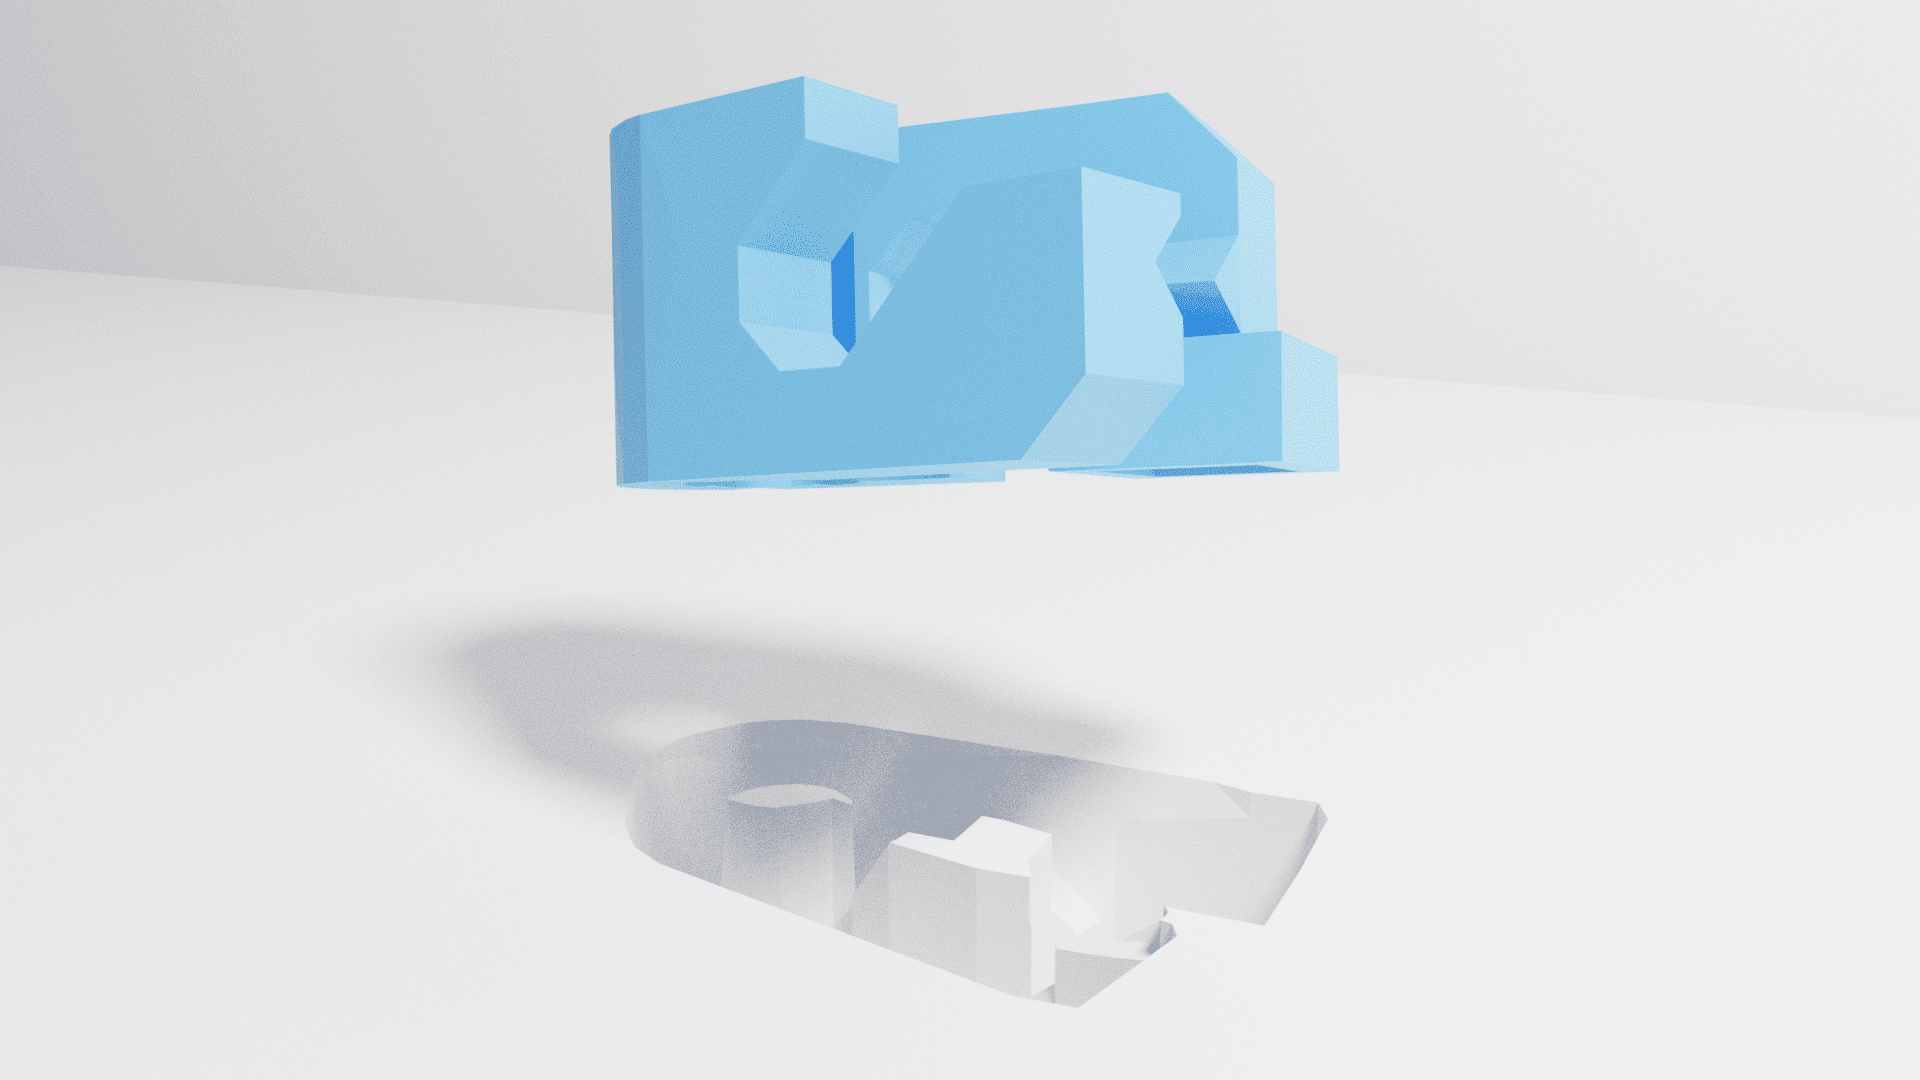
\includegraphics[width=121pt,trim=440 0 440 0, clip]{figures/bar_clamp_impression_2.png}\hfill%
  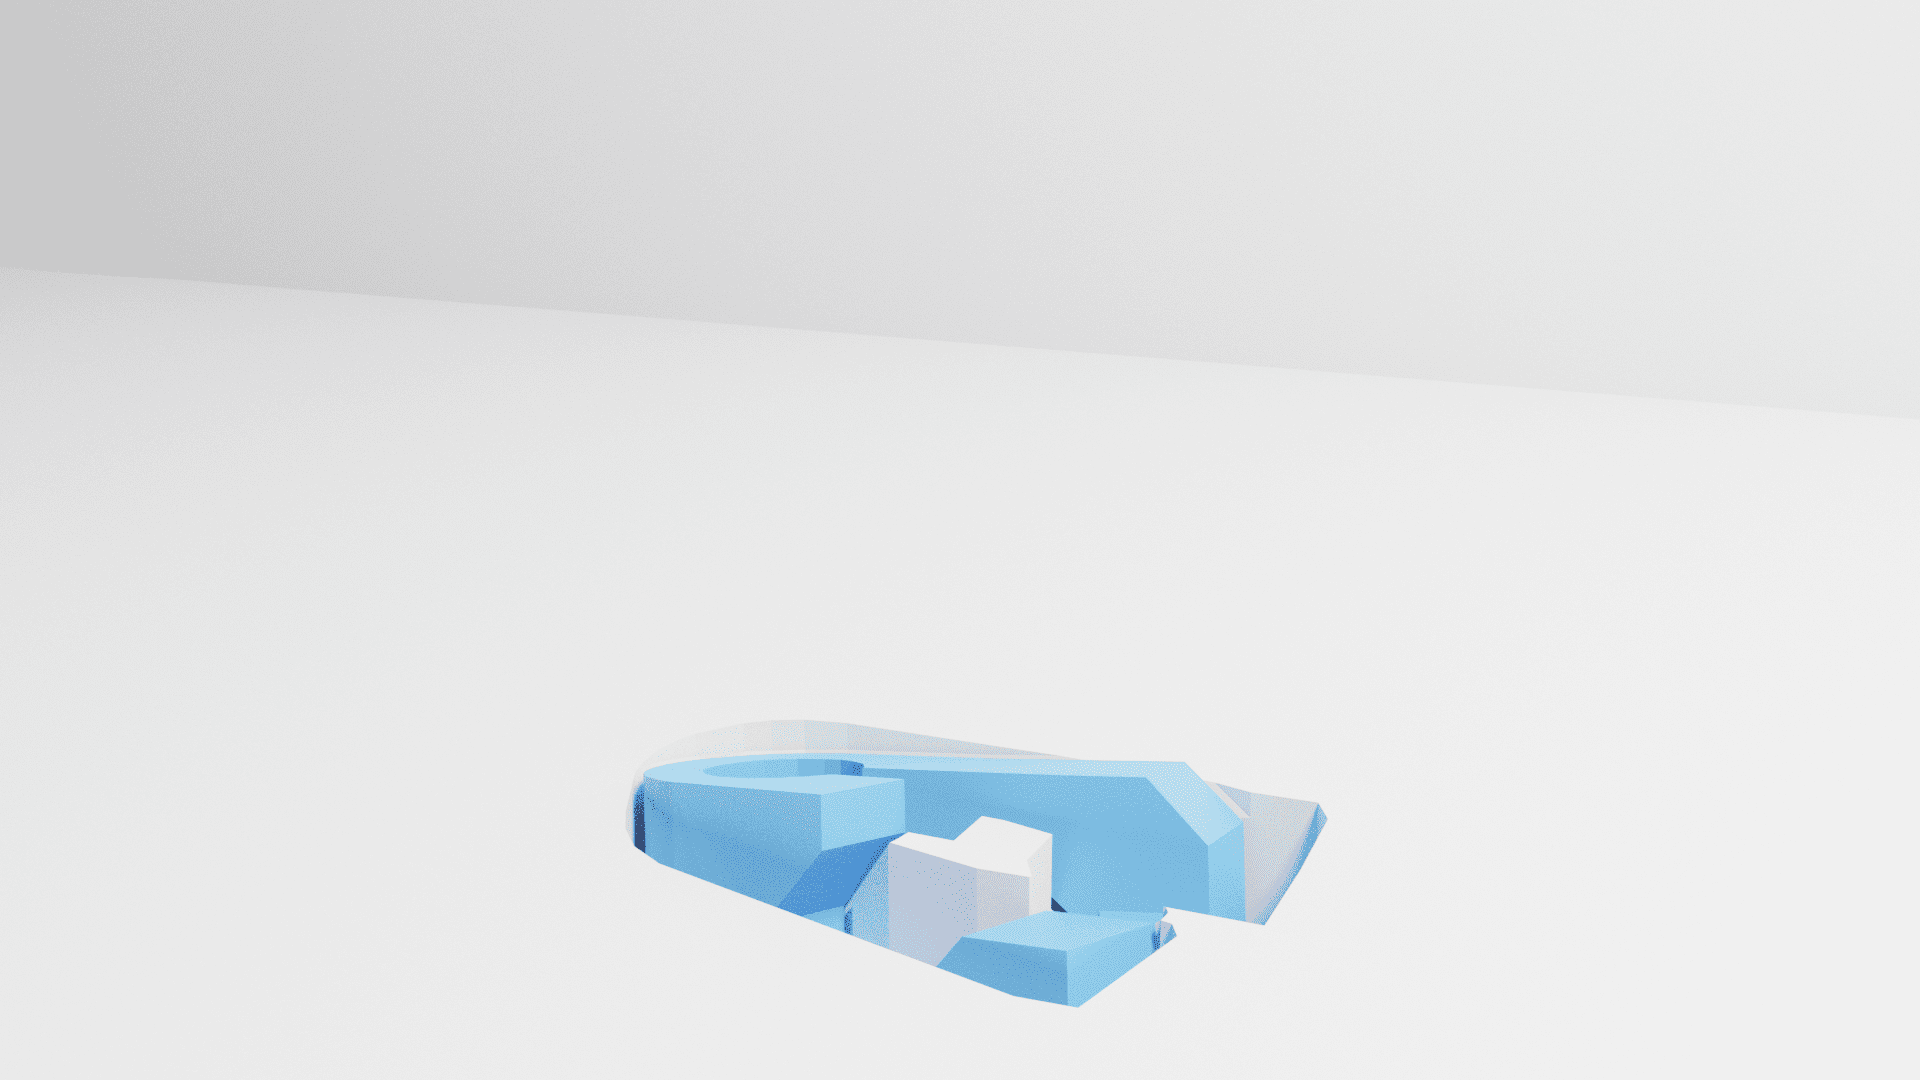
\includegraphics[width=121pt,trim=440 0 440 0, clip]{figures/bar_clamp_impression_4.png}
  \caption{\textbf{Successful Kitting: }Visualization of successfully kitting a 3D object into a concave cavity.}
  %\caption{\textbf{Generating Negative Goal Images: }Example an object (left) in a specific configuration $T^g$ and its complementary cavity created in simulation with Blender. We use the fatten operation to create a cavity with some slack for insertion (right). 
%   This cavity requires orienting the object to $\mathcal{G}$, a range of poses close to $T^g$ in order to be oriented.
  %}
  \label{fig:mug-cavity-2}
\end{figure}